\documentclass[12pt]{article}

\usepackage{amsmath}

\usepackage{graphicx}

\usepackage{hyperref} %querreferenzierung

\usepackage{xcolor}

\usepackage{amsmath} % for 'pmatrix' environment

\usepackage{listings} %code representation

\usepackage{trfsigns} %transformationszeichen

\usepackage{float} %floating images

\usepackage{subfig} %images next to one another

\usepackage{amssymb} %arrows

\usepackage{pdfpages} %add pdf to latex file

\usepackage{graphicx} %list of figures

\renewcommand*\contentsname{Inhaltsverzeichnis} % rename table of content

\renewcommand{\listfigurename}{Abbildungsverzeichnis}
\renewcommand{\listtablename}{Tabellenverzeichnis}

\usepackage{fancyhdr} %header and footer

% colored \pm
\usepackage{stackengine,xcolor}
\def\cpm{\mathbin{\ensurestackMath{\abovebaseline[-3.4pt]{%
				\stackunder[-3.5pt]{\color{green!70}+}{\color{red}-}}}}}

\usepackage[utf8]{inputenc}

\begin{document}
	\begin{titlepage}
		\centering
		\vspace{1cm}
		{\scshape\LARGE Hochschule Luzern \\ Technik und Architektur \par}
		\vspace{1cm}
		{\scshape\Large Bachelor Thesis\par}
		\vspace{1.5cm}
		{\huge\bfseries Entwicklung einer PCB zur Analyse von Umgebungslärm\par}
		\vspace{2cm}
		{\Large\itshape Stefano Nicora\par}
		
		\vfill
		
		% Bottom of the page
		{\large 7. Juni 2024\par}
	\end{titlepage}
	\tableofcontents
	
	%to do: add footer and header
	
	\newpage
	\section{Einleitung}
	\subsection{Ausgangslage} \label{Ausgangslage}
	Die Firma hEar hat es sich zum Ziel gesetzt, gegen \color{red}TODO\color{black}. Dazu wurde in der Masterarbeit von Sophie Mia Willener eine Marktanalyse durchgeführt, sowie ein erster Prototyp gebaut. Dieser Prototyp ist jedoch noch unhandlich und nicht für den Massenmarkt geeignet. 
	\subsection{Ziele} \label{Ziele}
	Das Ziel dieser Arbeit ist es, in einem ersten Schritt, auf Basis des vorhandenen Prototypen, ein funktionales, kompaktes und portables Schalldruckpegel-Messgerät zu entwickeln. Dabei sollen folgende Rahmenbedingungen zwingend eingehalten werden:
	\begin{itemize}
		\item Die Laufzeit des Gerätes soll mindestens 12 Stunden betragen.
		\item Das Gerät wird mit einem Akku betrieben. Dieser wird via eines USB-C-Anschlusses aufgeladen.
		\item Der Schalldruckpegel wird mit einem MEMS-Mikrofon aufgezeichnet.
		\item Die Messdaten werden in regelmässigen Abständen auf dem Gerät gespeichert.
		\item Das Gerät verfügt über eine BLE-Schnittstelle um die Messdaten drahtlos an ein Zielgerät zu übertragen.
		\item Der aktuelle Schalldruckpegel wird auf der Vorderseite des Gerätes visuell dargestellt.
	\end{itemize}
	In einem zweiten Schritt, wird das Gerät kalibriert und dessen Qualität mit auf dem Markt bereits vorhandenen Geräten verglichen.
	
	\newpage
	\section{Mikrofon}
	\subsection{Grundlagen}
	\subsubsection{MEMS}
	
	\subsubsection{I2S}
	Inter-Integrated Sound (I²S) bezeichnet eine Bus-Schnittstelle, welche von Philips zur Übertragung von digitalen Audiosignalen entwickelt wurde. Ähnlich wie I²C (Inter-Integrated Circuit) wird die Schnittstelle jedoch nur innerhalb des Gerätes verwendet. Dabei werden drei Pins zwischen Sender (hier das Mikrofon) und dem Empfänger (hier der Mikrocontroller) benötigt:
	\begin{itemize}
		\item \textbf{SCK} \quad (Serial Clock) \\
		Generiert die Taktrate, welche gleichzeitig die Datenrate der Übertragung definiert. Die Taktrate wird vom Master (hier der Mikrocontroller) vorgegeben.
		\item \color{green}\textbf{WS}\color{black} \quad (Word Select) \\
		Gibt vor, welcher Audiokanal (R, L) übertragen werden soll. Dies ermöglicht es, entweder ein Stereo-Signal oder zwei Mono-Signale wie zum Beispiel zwei Mikrofone zu übertragen.
		\item \color{red}\textbf{SD}\color{black} \quad (Serial Data)
		Beinhaltet den eigentlichen Datenstream mit der Datenrate definiert durch \textbf{SCK} und der Länge definiert durch \color{green}\textbf{WS}\color{black}.
	\end{itemize}
	\begin{figure}[H]
		\centering
		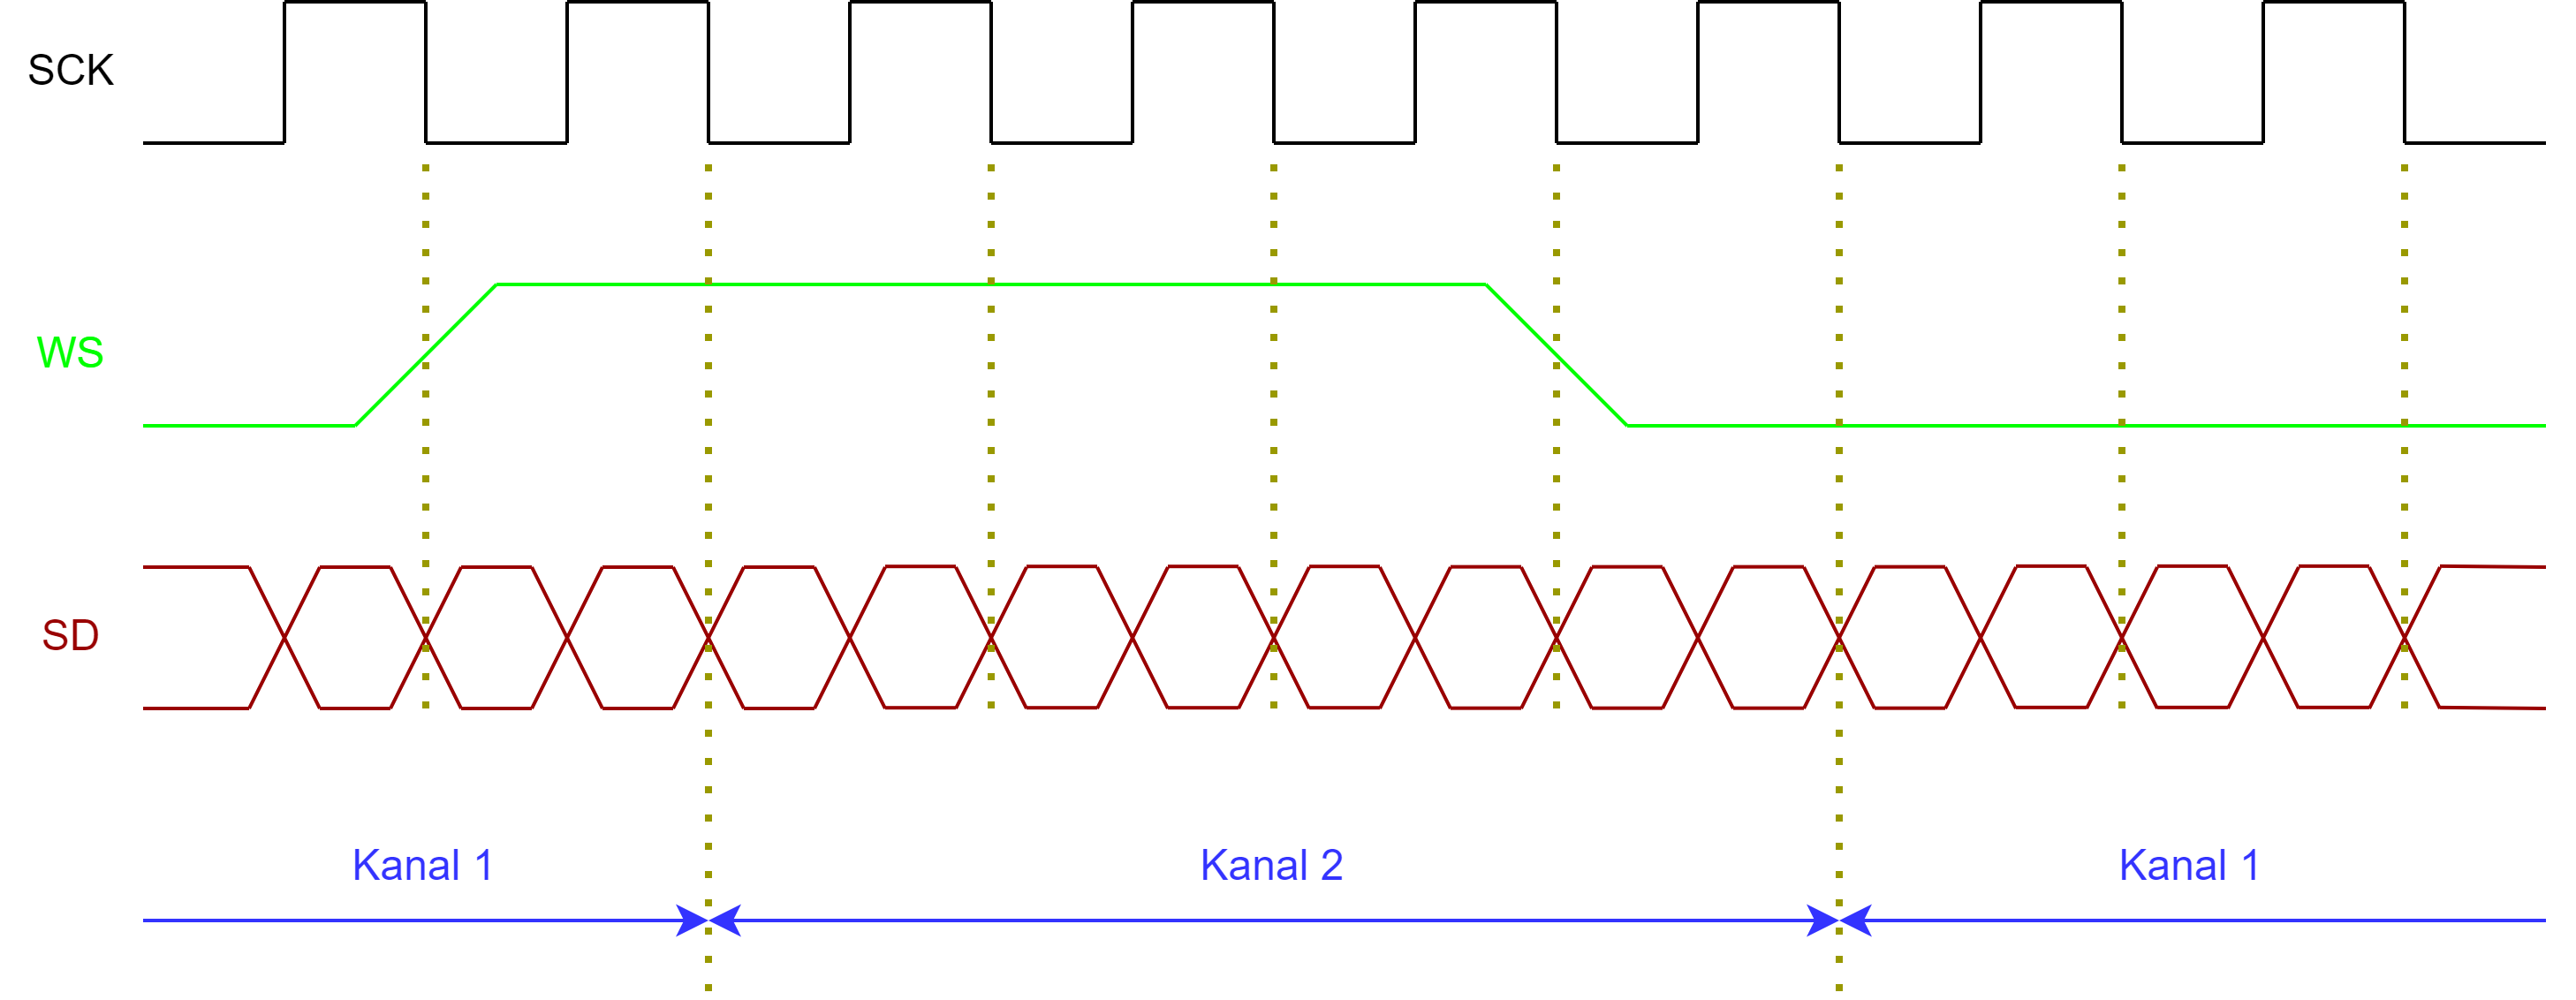
\includegraphics[width=1\linewidth]{images/BAT_I2S}
		\caption[]{Übersicht I2S-Signale}
		\label{fig:bati2s}
	\end{figure}
	\subsubsection{PDM}
	\textbf{P}ulse \textbf{D}ensity \textbf{M}odulation oder Pulsdichtemodulation bezeichnet die Darstellung eines analogen Signals in der digitalen Ebene. Dabei entspricht das Verhältnis zwischen der Anzahl der digitalen "1" und digitalen "0" der Amplitude des analogen Signales. Im Gegensatz dazu, wird im weit verbreiteten Pulsweitenmodulationsverfahren, kurz PWM, in jeder Periode das Verhältnis zwischen digitalem "1" und "0" variiert. Dies um zum Beispiel einen FET anzusteuern. \color{red}Farben von Bild anpassen\color{black}
	\begin{figure}[H]
		\centering
		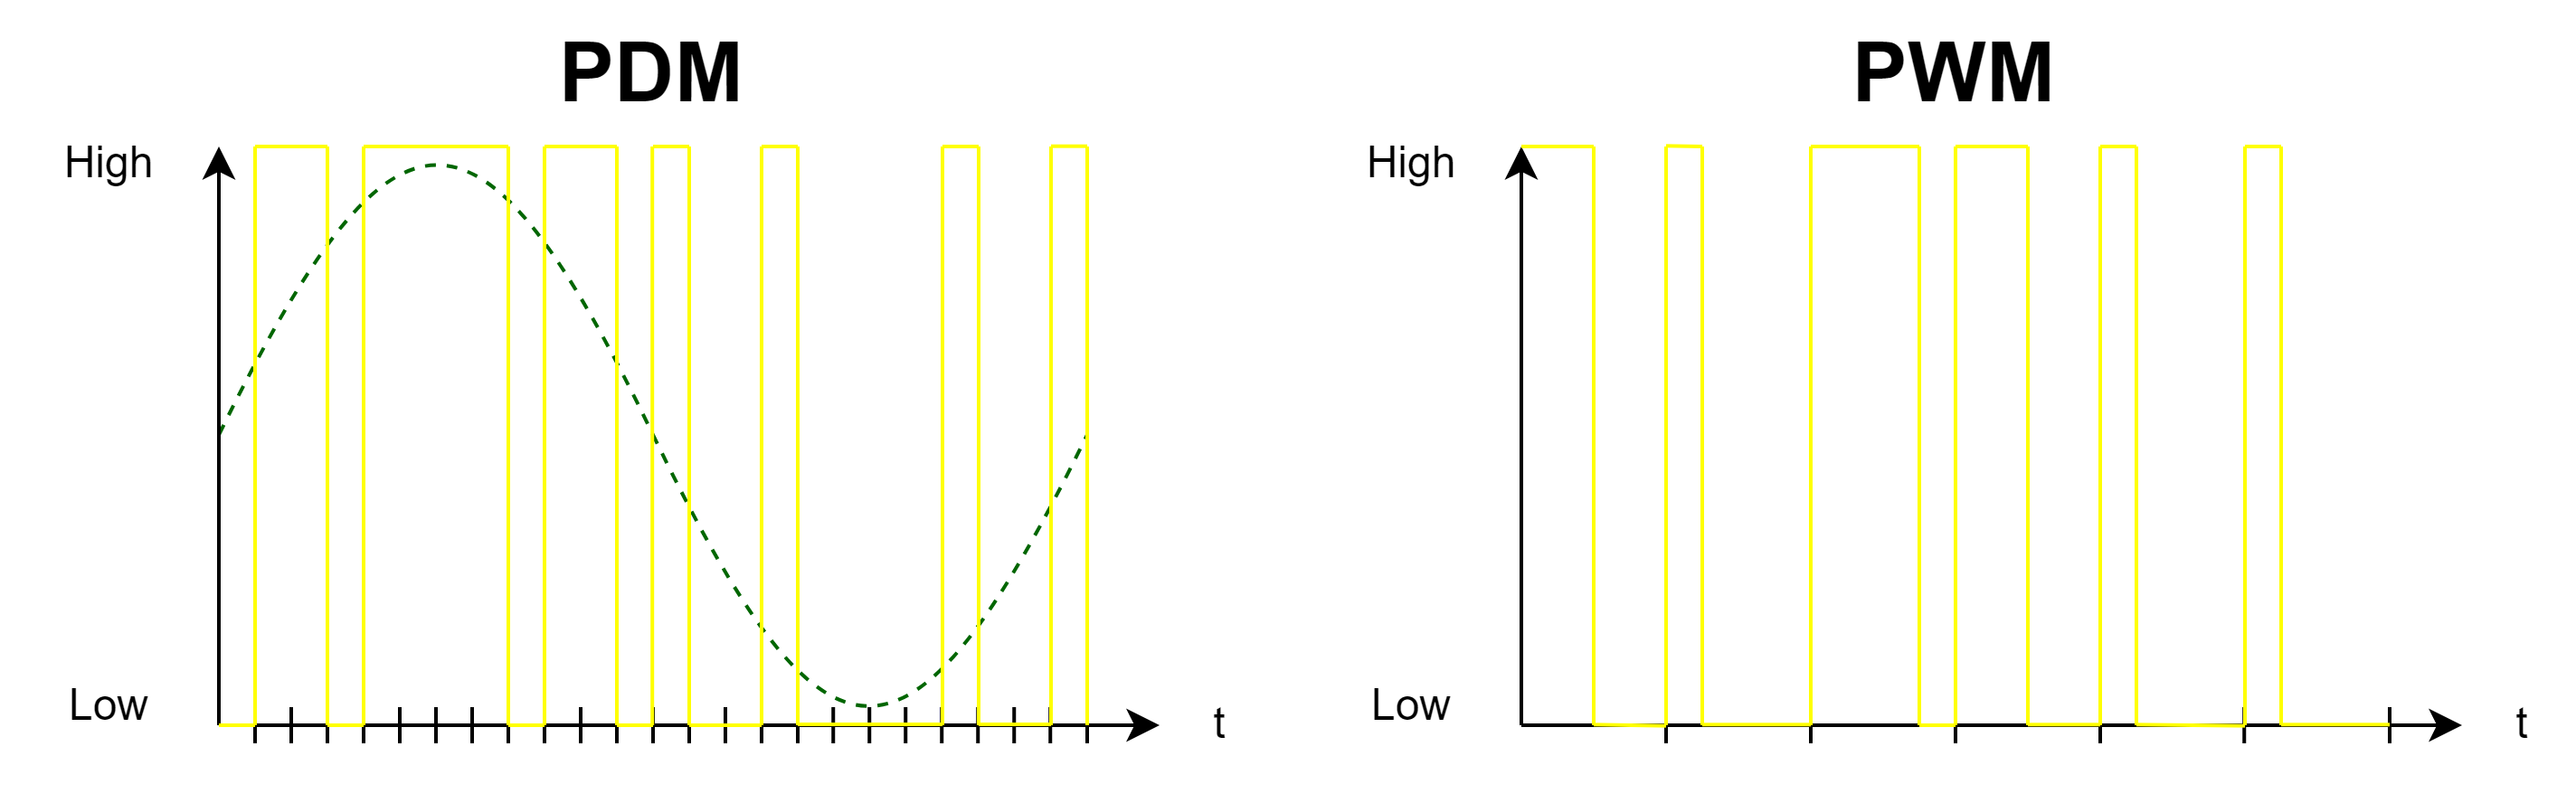
\includegraphics[width=1\linewidth]{images/BAT_PDM-vs-PWM}
		\caption{Vergleich PDM und PWM}
		\label{fig:batpdm-vs-pwm}
	\end{figure}
	
	\subsubsection{Schalldruckpegel}
	\subsubsection{Frequenzbewertung} \label{Frequenzbewertung}
	\subsection{Komponentenwahl}
	\subsubsection{Kriterien}
	\begin{itemize}
		\item Standort der Mikrofonöffnung
		\item Ausgangssignal
		\item Maximaler Schalldruckpegel
		\item MEMS-Technologie
		\item Frequenzbereich
	\end{itemize}
	\subsubsection{Vergleich}
	\subsubsection{Fazit}
	
	\newpage
	\section{Mikrocontroller}
	\subsection{Grundlagen}
	\subsubsection{DMA}
	Bei \textbf{D}irect \textbf{M}emory \textbf{A}ccess handelt es sich um eine Art Steuerbaustein, welcher unabhängig und parallel zum eigentlichen Rechenkern arbeitet. Dieser hat, wie der Rechenkern selbst, Zugriff auf den gesamten Datenbus. Dieser ermöglicht es, effizient Daten von Peripherien wie der UART, I²S, SPI, ect. in den RAM und umgekehrt zu laden. Dadurch wird der Rechenkern entlastet und kann für wichtigere Aufgaben eingesetzt oder gar in einen Energiesparmodus versetzt werden. Dabei gibt es zwei Möglichkeiten mit dem DMA-Baustein zu interagieren:
	\begin{itemize}
		\item Fire-and-forget
		\item \color{red}TODO\color{black}
	\end{itemize}
	\subsubsection{Bootloader}
	Unter einem Bootloader versteht man Code, welcher grundsätzlich nach dem erstmaligen flashen, persistent im System bleibt. Er dient als Ausgangspunkt für die eigentliche Software und ermöglicht es beispielsweise auch, während der Laufzeit des Gerätes, Softwareupdates herunter zu laden und diese anschliessend einzuspielen. Insbesondere wenn Funkprotokolle wie Bluetooth oder WLAN eingesetzt werden, ist ein Bootloader oftmals unerlässlich. Der Nachteil ist jedoch, dass dieser den ohnehin knappen Speicherplatz weiter reduziert.
	\subsubsection{RTC}
	Unter einer \textbf{R}eal \textbf{T}ime \textbf{C}lock versteht man ein Stück Hardware (intern oder extern), welche die Zeit ab Inbetriebnahme misst. Übliche RTCs haben, aufgrund ihrer Bauweise eine Genauigkeit von 100ppm. Da dies einer Zeitverschiebung von 4min und 19s @32kHz entspricht, enthalten die meisten RTCs Kompensationsmechanismen, um diese Zeit auf unter 100ms zu bringen. \cite{dighe_tps65950_2008}
% 	https://www.ti.com/lit/an/swca024/swca024.pdf?ts=1709375495514&ref_url=https%253A%252F%252Fwww.google.com%252F
	\subsubsection{Low Power}
	Mit Low Power wird, insbesondere bei Embedded-Systemen, die reduzierte Leistungsaufnahme beschrieben. Oftmals verfügen die Systeme über mehrere Modi mit jeweils unterschiedlichen Eigenschaften. Das Ziel ist es, mit jedem tieferen Modus etwas mehr Energie zu sparen und somit die Akkulaufzeit zu verlängern. Wie in Abbildung  \ref{fig:batlow-power-modestm} ersichtlich, sinkt zwar die Leistungsaufnahme mit jeder Stufe, jedoch werden dabei gewisse Peripherien abgeschaltet und die allgemeine Startzeit des Systems wird erhöht.
	\begin{figure}[H]
		\centering
		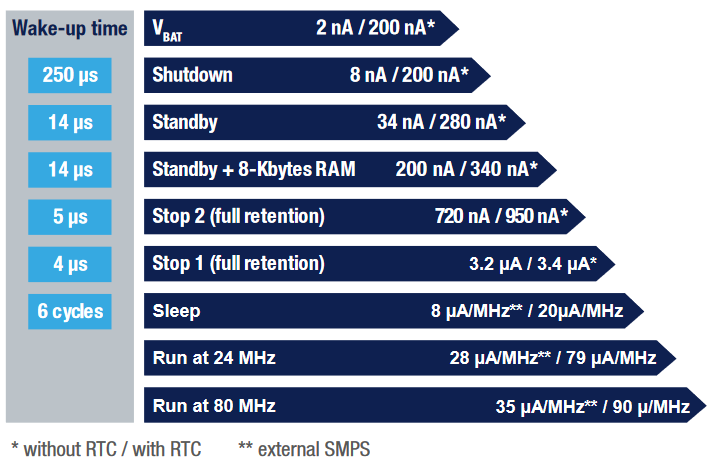
\includegraphics[width=0.7\linewidth]{images/BAT_Low-Power-Mode_STM}
		\caption{Vergleich Low-Power-Modi STM $\vert$ Quelle: \cite{noauthor_stm32l4_2024}}
		\label{fig:batlow-power-modestm}
	\end{figure}
	
	\subsubsection{Peripherie in Hardware oder Software}
	Bei allen gängigen Kommunikationsprotokollen ist die Frage, wie diese implementiert werden sollen. Dabei stehen folgende Möglichkeiten zur Auswahl:
	\begin{itemize}
		\item in \textbf{Hardware} \\
		+ Die benötigte Infrastruktur (Register, CRC, etc.) sind bereits physikalisch implementiert. Die Kommunikation kann dementsprechend vom Rechenkern abgekoppelt durchgeführt werden und ermöglicht eine gewisse Parallelität von mehreren Prozessen mit wenig Rechenaufwand. Insbesondere in Verbindung mit DMA, kann so viel Rechenzeit eingespart werden. \\
		- Bei den meisten Mikrocontrollern ist die spezifische Hardware an einzelne Pins gebunden. Dies wirkt sich auf die Flexibilität des PCB-Layouts oder gar des Gesamtsystems (zu wenig Anschlüsse) aus.
		\item in \textbf{Software} \\
		+ Die meisten Pins können flexibel für jedes Protokoll verwendet werden. Dadurch vereinfacht sich auch das PCB-Layouten.\\
		- Bei Verwendung von Ein-Kern-Systemen, welche im Embedded-Bereich mehrheitlich anzutreffen sind, kann keine echte Parallelität von Prozessen erfolgen. Dies verringert die Ausführungsgeschwindigkeit.
	\end{itemize}
	Grundsätzlich ist, nach Möglichkeit und Verfügbarkeit, eine Hardware-Peripherie zu bevorzugen. Insbesondere bei batteriebetriebenen Systemen mit langer Laufzeit, ist diese ausschlaggebend.
	\subsection{Komponentenwahl}
	Es existieren eine Vielzahl von Mikrocontroller-Herstellern. Viele dieser verfügen über eine breite Palette an BLE-tauglichen Chips. Um den geeignetsten darunter zu finden, werden nachfolgend die benötigten Schnittstellen definiert und mehrere, vorselektionierte Mikrocontroller, miteinander verglichen.
	\subsubsection{Kriterien}
	\begin{itemize}
		\item \textbf{I²S} + \textbf{PDM} zur Ansteuerung des Mikrofons.
		\item \textbf{SPI} zur Ansteuerung von möglichen Peripherien wie externe Speicherbausteine oder Displays.
		\item \textbf{I²C} zur Ansteuerung von Laderegler und LED-Treiber-IC.
		\item \textbf{DMA} zur energieeffizienten Verarbeitung der Daten.
		\item \textbf{RTC} um die gemessenen Werten mit einem Zeitstempel verknüpfen zu können.
		\item \textbf{BLE}-Fähiger Mikrocontroller mit vorgefertigter Antenne um die Integration zu vereinfachen.
	\end{itemize}
	\subsubsection{Vergleich}
	\begin{figure}[H]
		\centering
		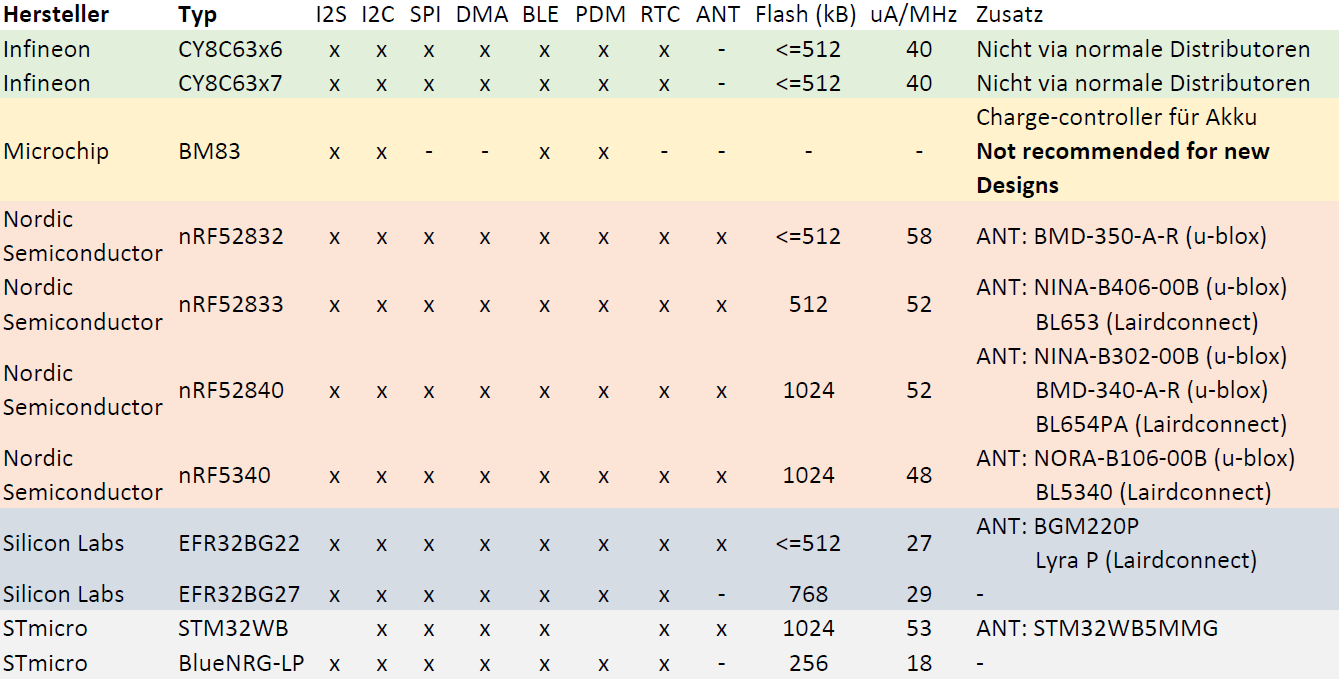
\includegraphics[width=0.9\linewidth]{tables/BAT_Vergleich-Mikrocontroller}
		\caption{Vergleich von möglichen Mikrocontrollern}
		\label{table:batvergleich-mikrocontroller}
	\end{figure}
	\subsubsection{Fazit}
	Wie dem Vergleich zu entnehmen ist, unterscheiden sich die Mikrocontroller meist nur in der integrierten Flash-Grösse sowie der Leistungsaufnahme bei einer gewissen Taktrate. Dadurch wird die Wahl nicht eingeschränkt, was eine geeignete Evaluation nicht vereinfacht. Ausschlaggebend ist jedoch der Formfaktor. Bis auf Silicon Labs und STmicro muss für einen Mikrocontroller mit vorgefertigter Antenne auf Drittanbieter ausgewichen werden. In Zeiten von Katastrophen wie COVID oder Kriegen inmitten von Handelsrouten ist die Produktverfügbarkeit einer der zentraler Aspekte. Aus diesem Grund wird nachfolgend der EFR32BG22 von Silicon Labs bzw. dessen Modul-Variante, der \textbf{BGM220P}, eingesetzt.
	
	\newpage
	\section{LED}
	\subsection{Grundlagen}
	\subsubsection{Wellenlänge}
	\subsubsection{Leistungsaufnahme}
	\subsubsection{Lichtleistung}
	\subsubsection{Vorwiderstand / Strombegrenzung}
	\subsection{Komponentenwahl}
	\subsubsection{Kriterien}
	\begin{itemize}
		\item Lichtleistung 
		\item Wellenlänge
	\end{itemize}
	\subsubsection{Vergleich}
	
	\newpage
	\section{Entwicklung}	
	\subsection{Konzept}
	Die im Unterkapitel \ref{Ziele} definierten Ziele sollen nun umgesetzt werden. Dazu soll die von aussen sichtbare Vorderseite möglichst wenig Bauteile aufweisen, um das visuelle Design nicht zu beeinträchtigen. Mit einer angestrebten Gesamtgrösse von 60mm Durchmesser, können die gewählten Bauteile geradenoch auf dem PCB in einer symmetrischen Art platziert werden. 
	\paragraph{Front}
	Die Vorderseite weist folgende Bauteile auf:
	\begin{itemize}
		\item 8 LEDs
		\item Mikrofon
		\item LED-Treiber-IC
	\end{itemize}
	Zudem sind die LEDs sind ringförmig angeordnet, um der Anforderung eines visuellen Ladebalkens entsprechen zu können.
	\paragraph{Back}
	Die Rückseite hingegen, beinhaltet folgende Bauteile:
	\begin{itemize}
		\item USB-C-Ladeanschluss
		\item Polyfuse (Automatisch rückstellbarer Überstromschutz)
		\item Switch um generell das Gerät ein- und auszuschalten
		\item BMS, um den Akku sicher auf- und entladen zu können
		\item Mikrocontroller, welcher sich aufgrund seiner Antenne am Rand des PCBs befinden muss
		\item Akkuhalter
		\item Optionaler Speicherbaustein
	\end{itemize}
	\begin{figure}[H]
		\centering
		\includegraphics[width=0.9\linewidth]{images/BAT_Konzept_Gerät}
		\caption{Konzept PCB-Layout}
		\label{fig:batkonzeptgerat}
	\end{figure}
	\begin{figure}[H]
		\centering
		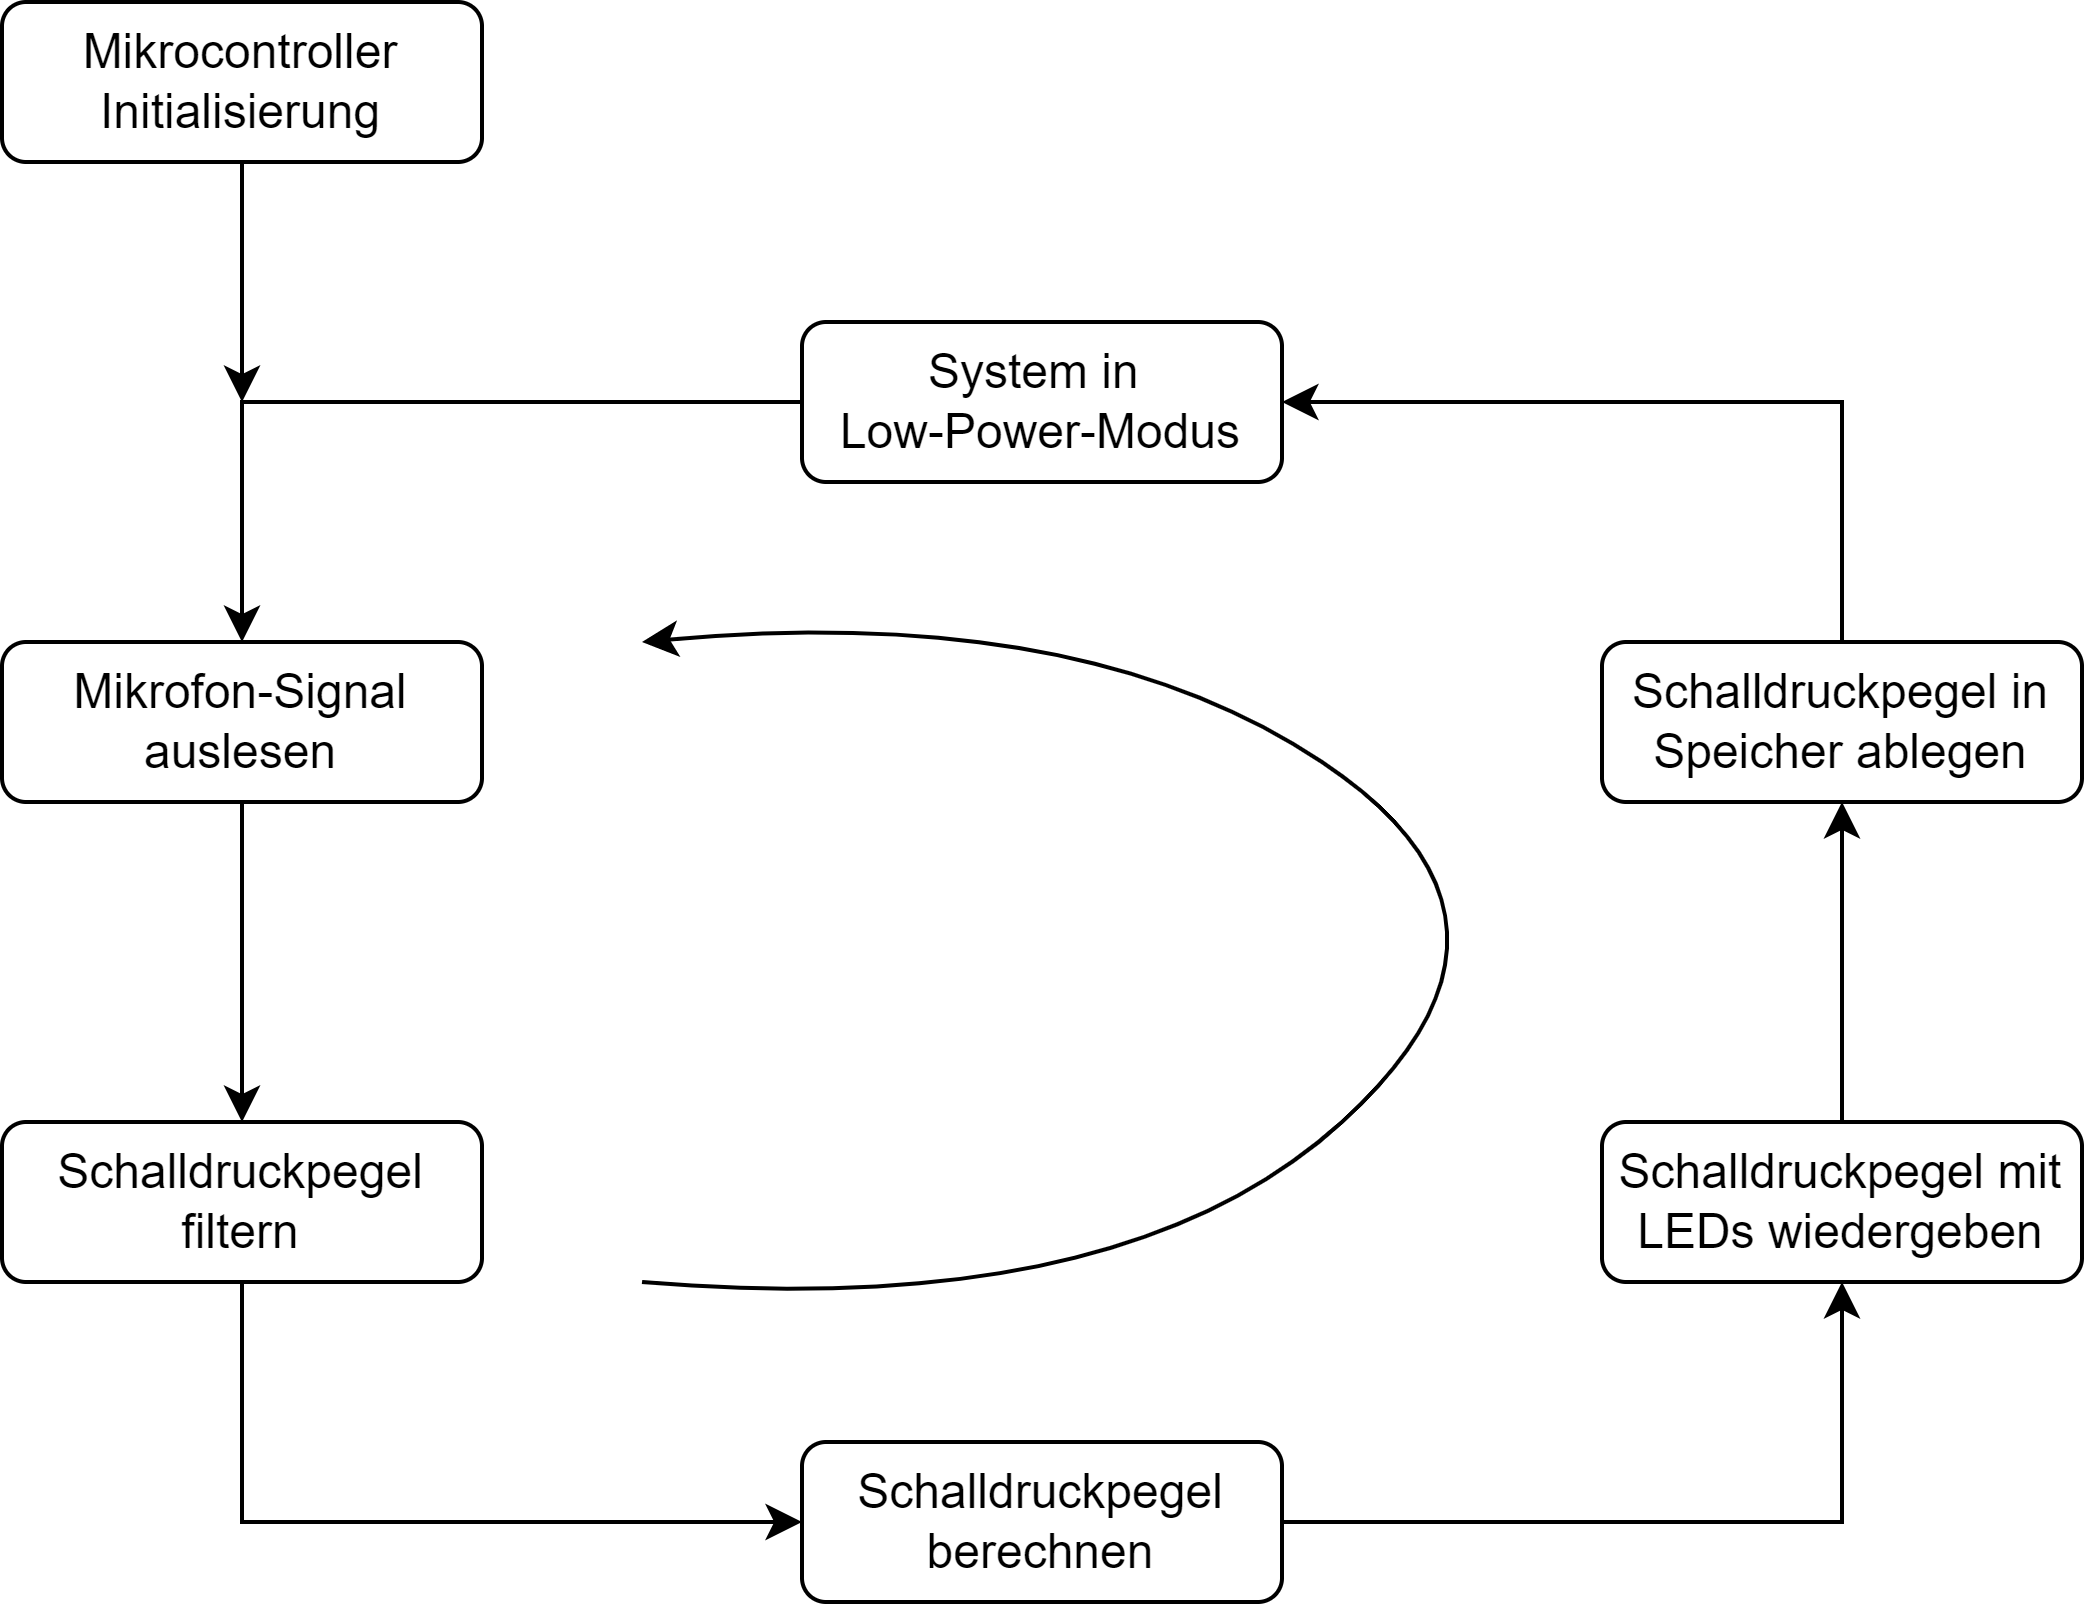
\includegraphics[width=0.9\linewidth]{images/BAT_Konzept_Softwareablauf}
		\caption{Konzept Softwareablauf}
		\label{fig:batkonzeptsoftwareablauf}
	\end{figure}
	
	\subsection{Hardware}
	\subsubsection{PCB}
	\paragraph{Laderegler}
	\subsubsection{Kosten}
	\subsection{Software}
	\subsubsection{Filterdesign}
	Wie im Unterkapitel \ref{Frequenzbewertung} erläutert, reagiert unser Gehör nicht auf alle Frequenzen gleich. Um diese Frequenzbewertung in die Schalldruckpegel-Berechnung einfliessen zu lassen, wird ein digitales, diskretes Filter benötigt. Die benötigten Frequenzbewertungsfilter werden jedoch fast ausschliesslich in der S-Ebene (Laplace-Bereich, zeitkontinuierlich) veröffentlicht. Dadurch müssen diese mit der bilinaren Transformation \cite{oppenheimer_alan_v_zeitdiskrete_nodate} vom Frequenz- in den Zeitbereich transformiert werden.
	\begin{equation}\label{G_A_s}
		G_A(s) = \frac{7.39705 \cdot 10^9 \cdot s^4}{(s+129.4)^2\cdot (s+676.7)\cdot (s+4636)\cdot (s+76617)^2}
	\end{equation}
		\begin{equation}\label{G_C_s}
		G_C	(s) = \frac{5,91797 \cdot 10^9 \cdot s^2}{(s+129,4)^2\cdot (s+76617)^2}
	\end{equation}
	
	\subsubsection{PDM}
	\subsubsection{I²C}
	\subsubsection{SPI}
	
	\newpage
	\section{Messungen}
	\subsection{Leistungsaufnahme}
	\subsection{Mikrofon-Kalibrierung}
	\subsection{Vergleich}
	
	\newpage
	\section{Fazit und Ausblick}
	
	\newpage
	\section{Anhang}
	\bibliography{Sources} 
	\bibliographystyle{ieeetr}
	\listoffigures
	\subsection{Fremdwörter}
	CRC \\
	Register \\
	Pins \\
	Embedded \\
	ppm \\
	flashen \\
	
	
	
\end{document}